\documentclass[12pt]{article}

\usepackage{geometry}
\geometry{paper=letterpaper, top=1in, bottom=1in, left=1in, right=1in}

\usepackage{amsmath, amsfonts, amssymb}

\usepackage{physics}

\usepackage{graphicx}
% Title Page
\title{CI Nets, Software Preferences and Quantum Computing}
\author{Scott J. Schoeller\\UW--Whitewater}
\date{}


\begin{document}
\pagenumbering{gobble}
\maketitle

\newpage
\begin{flushleft}
\section{Introduction}
\subsection{Conditional Importance Networks}
Conditional Importance networks are a type of graph that are formed from a set of conditional importance statements. The following definitions are adapted from Oster et al. \cite{  oster_efficient_2017, oster_scalable_2015}.\\

\subsubsection*{Definition 1. CI statements}
A CI statement on $\mathbf{V}$ is a quadrapole $(S^+ ,S^-, S_1, S_2)$ that is expressed as pair-wise, disjoint subsets of $\mathbf{V}$.
A CI statement can be written as follows:
\small
\begin{equation*}
S^+, S^- : S_1 \vartriangleright S_2 
\end{equation*}
or alternatively, as:
\begin{equation*}
\{True-conditions \}, \{False-conditions \}: \{more-preferred-items \} \succ \{less-preferred-items \}
\end{equation*}
\normalsize

\subsubsection*{Definition 2. CI networks}
A CI network, $\mathbf{C}$, over a set of variables $\textbf{V}$ is satisfiable if and only if there exists a strict partial order over the powerset of $\mathbf{V}$ such that:\\
1. For each CI-net statement $S^+$, $S^{-}$: $S_1 \vartriangleright S_2$, if $S \subseteq V /\ (S^+ \cup S^- \cup S_1 \cup S_2)$, then $S \cup S^+ \cup S_1 \succ S \cup S^+ \cup S_2$\\
2. $\succ$ is monotonic (for any $V_i, V_j \subseteq \mathbf{V}$, $V_i  \supset  V_j,  V_i \succ V_j$)

\subsubsection{Software Engineering Preferences}
Software engineering preferences, which are a preferred set of features in a computer software product, can be expressed as CI networks.

\subsubsection{Importance as a Partial Ordering}
I make the contribution of ``importance of preferences", or ``importance" for short, as a partial ordering. The preference that occurs the most is considering the required feature and the others are ordered with possible ties in descending order of preference. This is in contrast to the original CI network approach, which requires a strict partial ordering \cite{oster_scalable_2015}.

\subsection{Quantum Computing}
Quantum computing is an alternative computing paradigm attributed to Richard Feynmann and Yuri Manin. Quantum computers utilize quantum particles to have the properties of quantum systems. Another benefit to this model is the potential for polynomial-time solutions to otherwise exponential problems. The class of problems solvable by a quantum computer is known as BQP, which encompasses all problems solvable by a classical computer in polynomial time and additional problems that can only be broken in polynomial time on a quantum computer. Quantum computers are non-deterministic.
\subsubsection{Tool for Combinatorial Problems}
The quantum computing paradigm is useful for combinatorial problems such as graph search.
\subsubsection{Grover's Search Algorithm}
Grover's Algorithm is a quantum search algorithm. This runs in $O(\sqrt{N})$ time instead of $O(N)$ time as would be the case for a classical computer.

\section{Methods}
The quantum triangle algorithm \#3 in a MSc thesis was used \cite{cirasella_classical_2006, cirasella_classical_2006-1}. The only modifications were not using randomization prior to Grover's Algorithm due to how IBM expects the input. The output was manually interpreted for the most likely outcome. Each qubit in a four qubits grouping represented $d,c,b,a$, or $v_0$ to $v_3$ as provided in Fig. 1.\\
\ \\
% Figure 1
\begin{figure}[h!]
\begin{center}
0~~0~~0~~0\\
$d$~~$c$~~$b$~~$a$\\
$v_3$ $v_2$ $v_1$ $v_0$
\end{center}
\caption{Qubit values and interpretation}
\end{figure}
The following CI statements were used:\\
\begin{figure}[h!]
\begin{center}
\{$d$\};\{\}:\{$b$\};\{$c$\}\\
\{$b$\};\{$a$\}:\{$c$\};\{$d$\}\\
\{\};\{$d$\}:\{$a,b$\};\{$c$\}
\end{center}
\caption{Simple CI statements}
\end{figure}

\begin{figure}[h!]
	\begin{center}

\{$v_2$\};\{\}:\{$v_3$\};\{$v_1$\}\\
\{\};\{\}:\{$v_0$\};\{$v_1$\}\\
\{\};\{\}:\{$v_3$\};\{$v_0$\}\\
\{\};\{$v_0,v_2$\}:\{$v_3$\};\{$v_1$\}\\
\{\};\{\}:\{$v_2$\};\{$v_1$,$v_3$\}\\
\{\};\{$v_3$\}:\{$v_0$\};\{$v_1$\}\\
\{$v_0$\};\{$v_3$\}:\{$v_1$\};\{$v_2$\}

	\end{center}
	\caption{Complex CI statements}
\end{figure}

\begin{figure}
\begin{center}
\{$a$\};\{\}:\{$b$\};\{$c$\}\\
\{$b$\};\{$a$\}:\{$c$\};\{$d$\}\\
\{\};\{$d$\}:\{$c$\};\{$a,b$\}

\end{center}
\caption{Inconsistent CI statements}
\end{figure}

\section{Results}
% Figure 2
\ \\
\begin{figure}[h!]
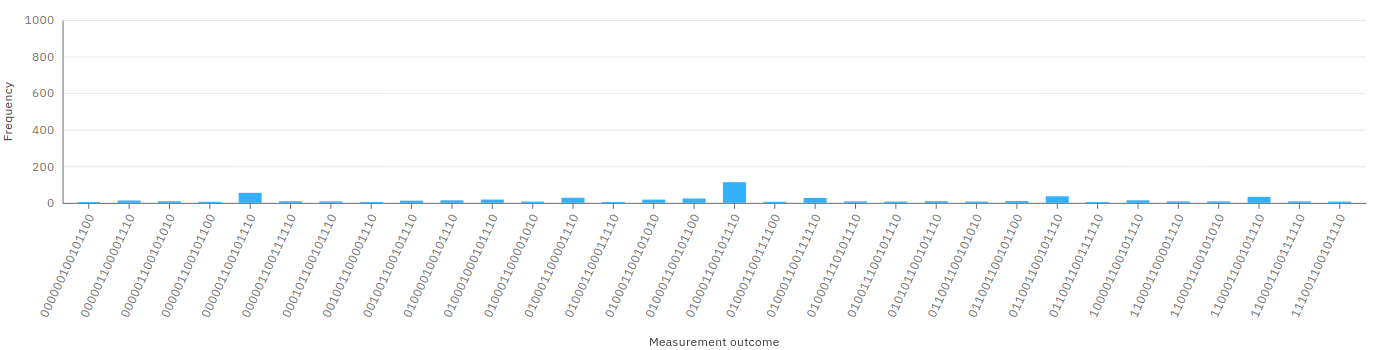
\includegraphics[width=\linewidth]{chart1.png}
\caption{Simplest CI-net}
\label{cinet:simple}
\end{figure}
\par{The raw result was: 0100 0110 0101 1100.
The interpretation of the first result is that c is the most important attribute, while a,b and d have equal importance.\\
The runtime was 12.7 seconds.}
\ \\
% Figure 3
\begin{figure}[h!]
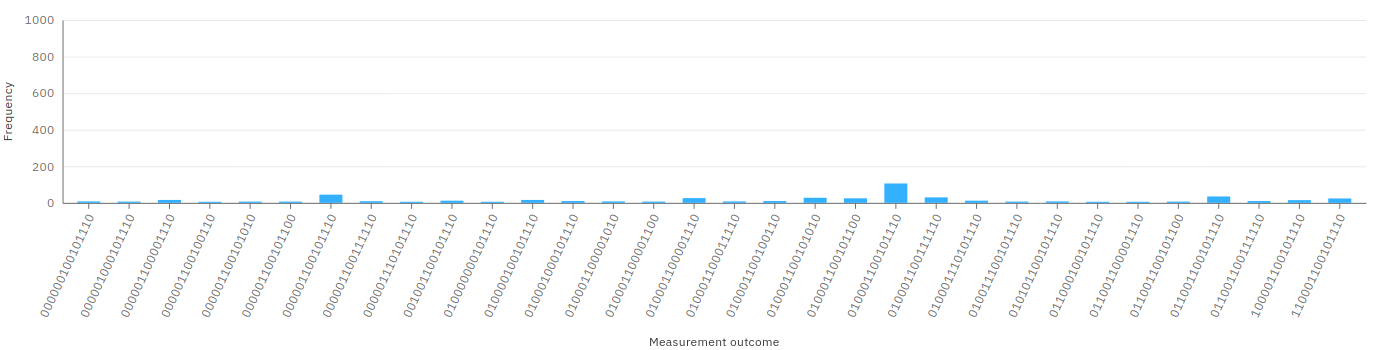
\includegraphics[width=\linewidth]{chart2.png}
\caption{Complex CI-net}
\label{cinet:complex}
\end{figure}
\ \\
\par{The raw result was: 0100 0110 0101 1110.
The interpretation of the second result is that $v_2$ is the most important attribute, followed by $v_1$ and $v_3$. The runtime was 12.8 seconds.}

\par{
The final CI-net was considered unsolvable if analyzed by the previous approach. The quantum algorithm was able to break the cycle and returned results after a 13.3 second runtime.}
\begin{figure}[h!]
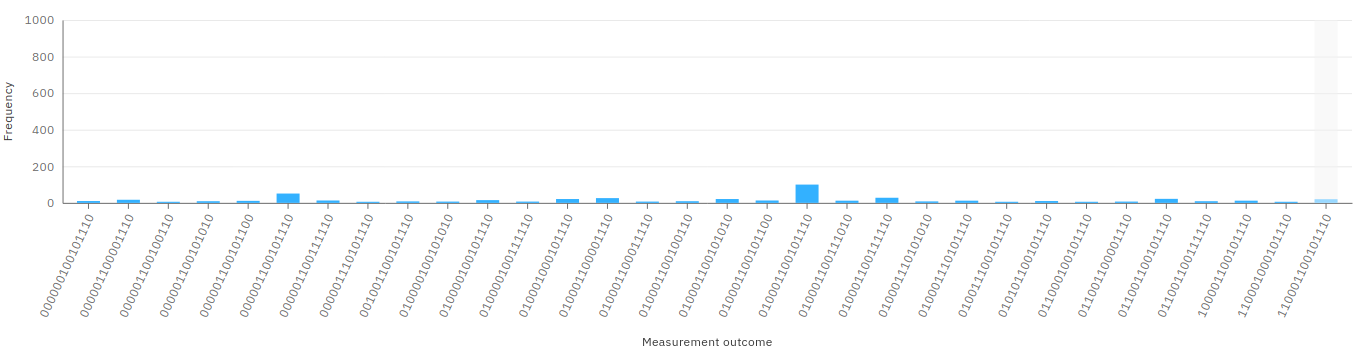
\includegraphics[width=\linewidth]{chart3.png}
\caption{Previously unsolvable CI-net}
\end{figure}
\ \\
The primary result returned is:\\
0100 0110 0101 1110\\
~$v_2$~~~$v_1,v_2$~~$v_0,v_2$~$v_1,v_2,v_3$\\
$v2$ is the most important preference, followed by $v_1$ and $v_0/v_3$ (tie).

\newpage

\section{Conclusion}
% Meaning of results
For the simplest case (Fig. \ref{cinet:simple}), the results were verified manually as a solution. The algorithm was assumed accurate for the more complex case (Fig. \ref{cinet:complex}).
What were previously unsolvable statements if analyzed as a pure CI network can potentially be deemed solvable with this new approach utilizing partial orderings.
The efficiency of this quantum computing approach is expected to grow as more powerful computers of this type are manufactured. Some of the time also includes communication delays between the host system and the quantum computer.

\section{Acknowledgments}
Thanks to IBM for making their Quantum Experience readily available. Gratitude is also extended to the following people: Dr. Donald Knuth and Dr. Zach Oster.

\newpage
\bibliography{CInets.bib}
\bibliographystyle{acm}

\end{flushleft}

\end{document}